\subsection{Organization of phonemes}
\label{sec:organization}

In this section we take a closer look at the underlying organization
of phonemes in the model.  Our experiment is inspired by 
\citet{khalighinejad2017dynamic} who study how
the speech signal is represented in the brain at different stages of
the auditory pathway by collecting and analyzing electroencephalography 
responses from participants listening to continuous speech, and show that brain
responses to different phoneme categories turn out to be organized by
phonetic features. 
%They compared the patterns of phoneme
%similarity in the neural responses and the acoustic signals and
%demonstrated that acoustic distinctions of phonemes are reflected in
%the corresponding neural data.

%{\it I assume most of the following paragraph will move to introduction or related work, but I keep it here 
%for now to motivate the experiment. Also most of the content is copied from their paper, so we need to 
%rewrite the text.}
%
%To study how the speech signal is represented in the brain at different stages of the auditory pathway, 
%\cite{khalighinejad2017dynamic} collected electroencephalography responses to continuous speech by 
%obtaining the time-locked responses to phoneme instances (phoneme-related potential), and showed 
%that responses to different phoneme categories are organized by phonetic features. In addition, they 
%compared the patterns of phoneme similarity in the neural responses and the acoustic signals which 
%showed a repetitive appearance of acoustic distinctions of phonemes in the neural data. Their analysis 
%of the phonetic and speaker information in neural activations revealed that different time intervals jointly 
%encode the acoustic similarity of both phonetic and speaker categories. 

%Here we present a simulation of the study of \cite{khalighinejad2017dynamic} by analyzing the hidden 
%layer activations of our model in response to each phoneme in the input, and compare them to the 
%MFCC representations of these phonemes in the speech signal. 
%
%The phoneme activations in each layer, which can be thought as the model's equivalent to the phoneme-
%related potentials, and are calculated as the hidden layer activations averaged over the duration of the 
%phoneme token in the input. The average input vectors are similarly calculated as the MFCC vectors 
%averaged over the time course of the articulation of the phoneme token. Each phoneme type is 
%represented by the average input vector of all its instances in the validation set, and the average 
%activation vector of all its instances for each hidden layer in the model.
%
%%\subsubsection{Correlation with audio representations}
%
%Following \cite{khalighinejad2017dynamic}, we generated a distance matrix for every pair of phonemes 
%by calculating the euclidean distance between the phoneme pair's activation vectors for each layer 
%separately. Similarly, we calculated the distance matrix for the audio vectors of all phoneme pairs in our 
%data. We then calculated the Pearson correlations between the lower triangular part the audio distance 
%matrix and each of activation distance matrix for each layer. 
%\todo{Check that this is what we are doing.}
%>>>>>>> 5719ea4ce48084d7f0d6f9416d2c278836afbc8f



\begin{figure}[t]
  \centering
  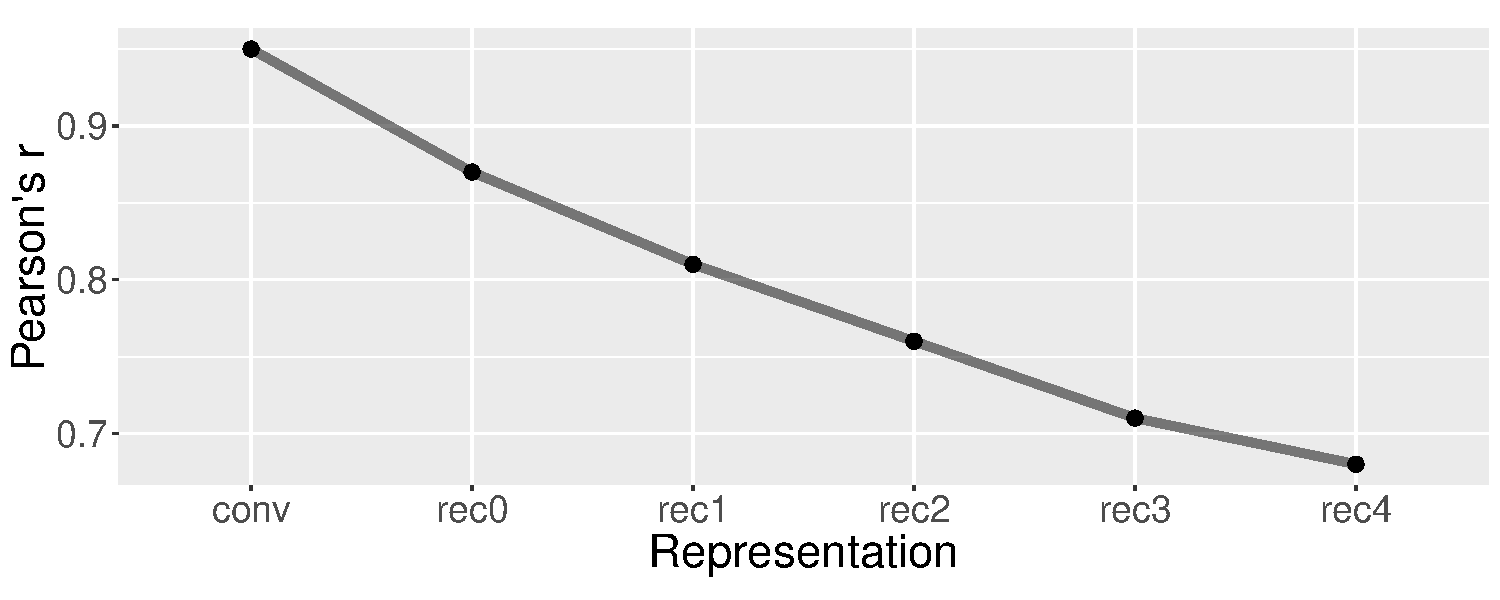
\includegraphics[scale=0.28]{figures/correlation_mfcc.pdf}
  \caption{Pearson's correlation coefficients $r$ between the distance matrix of MFCCs and distance matrices on activation vectors.}
  \label{fig:correlation}
\end{figure}


% Convolutional & 0.95 \\
% Layer 1 &  0.87 \\
% Layer 2 &  0.81 \\
% Layer 3 &  0.76 \\
% Layer 4 &  0.71 \\
% Layer 5 &  0.68 \\



We carry out an analogous experiment by analyzing the hidden layer activations of our model in 
response to each phoneme in the input. First, we generated a distance matrix 
for every pair of phonemes by calculating the Euclidean distance between the 
phoneme pair's activation vectors for each layer separately, as well as a 
distance matrix for all phoneme pairs based on their MFCC features. Similar to 
what \citet{khalighinejad2017dynamic} report,  we observe that the phoneme 
activations on all layers significantly correlate with the phoneme representations 
in the speech signal, and these correlations are strongest for 
the lower layers of the model. Figure~\ref{fig:correlation} shows the results.

%The phoneme activations in each layer, which can be thought as the model's 
%equivalent to the phoneme-
%related potentials, and are calculated as the hidden layer activations 
%averaged over the duration of the 
%phoneme token in the input. The average input vectors are similarly 
%calculated as the MFCC vectors 
%averaged over the time course of the articulation of the phoneme token. Each 
%phoneme type is 
%represented by the average input vector of all its instances in the validation 
%set, and the average 
%activation vector of all its instances for each hidden layer in the model.
%
%\subsubsection{Correlation with audio representations}


%\subsubsection{Organization of phonemes}
%\label{sec:clustering}

%\begin{table*}
%\caption{Evaluation of phoneme clusters based on audio features and layer 
%activations.}
%\label{tab:clustering}
%\begin{center}
%\begin{tabular}{c|c|c|c|c}
%&	{\bf Rand Index}& {\bf Homogeneity} & {\bf Completeness} & {\bf V-
%measure} \\
%\hline
%Audio features		& 0.27		& 0.59		& 0.52		& 0.55 \\
%Activations layer 0	& 0.23		& 0.47		& 0.45		& 0.46 \\
%Activations layer 1	& 0.16		& 0.47		& 0.45		& 0.46 \\
%Activations layer 2	& 0.16		& 0.47		& 0.45		& 0.46 \\
%Activations layer 3	& 0.15		& 0.43		& 0.48		& 0.45 \\
%Activations layer 4	& 0.15		& 0.43		& 0.48		& 0.45 \\
%\hline
%\end{tabular}
%\end{center}
%\end{table*}

%phone mode: short	activation mode: avg
%
%Clustering		Rand Index	Homogeneity	Completeness	V-measure
%Audio features	        0.27		0.59		0.52		0.55
%Conv. activations	0.12		0.44		0.40		0.42
%Activations layer 0	0.23		0.47		0.45		0.46
%Activations layer 1	0.16		0.47		0.45		0.46
%Activations layer 2	0.16		0.47		0.45		0.46
%Activations layer 3	0.15		0.43		0.48		0.45
%Activations layer 4	0.15		0.43		0.48		0.45
%
%---------
%
%phone mode: long	activation mode: avg
%
%Clustering		Rand Index	Homogeneity	Completeness	V-measure
%Audio features		0.18		0.45		0.42		0.44
%Conv. activations	0.20		0.43		0.41		0.42
%Activations layer 0	0.16		0.43		0.40		0.41
%Activations layer 1	0.11		0.39		0.39		0.39
%Activations layer 2	0.11		0.40		0.38		0.39
%Activations layer 3	0.06		0.33		0.38		0.35
%Activations layer 4	0.06		0.28		0.32		0.30

%% \begin{figure*}[t]
%%   \centering
%%   \includegraphics[scale=0.37]{figures/audio.png}
%% \caption{Hierarchical clustering of phoneme audio vectors.}
%% \label{fig:cluster-audio}
%% \end{figure*}
%% \begin{figure*}[t]
%%   \centering
%%   \includegraphics[scale=0.37]{figures/activation4.png}
%% \caption{Hierarchical clustering of phoneme activation vectors on the last 
%%  hidden layer.}
%% \label{fig:cluster-l4}
%% \end{figure*}
We then performed agglomerative hierarchical clustering on phoneme type MFCC and 
activation vectors, using Euclidean distance as the distance metric and the Ward linkage criterion \citep{ward1963hierarchical}.
%We compared the class labels extracted from the clustering tree to a set of 
%manually-annotated gold-standard labels for phoneme categories. 
%Table~\ref{tab:clustering} shows the clustering results.
Figure~\ref{fig:cluster-l0} shows the clustering results for the activation vectors
on the first hidden layer. The leaf nodes are color-coded according to phoneme classes as specified in Table~\ref{tab:phoneme-list}. There is substantial degree of matching between the classes and the structure of the hierarchy, but also some mixing between rounded back vowels and voiced plosives /b/ and /g/, which share articulatory features such as lip movement or tongue position. 
\begin{figure}[ht]
  \centering
  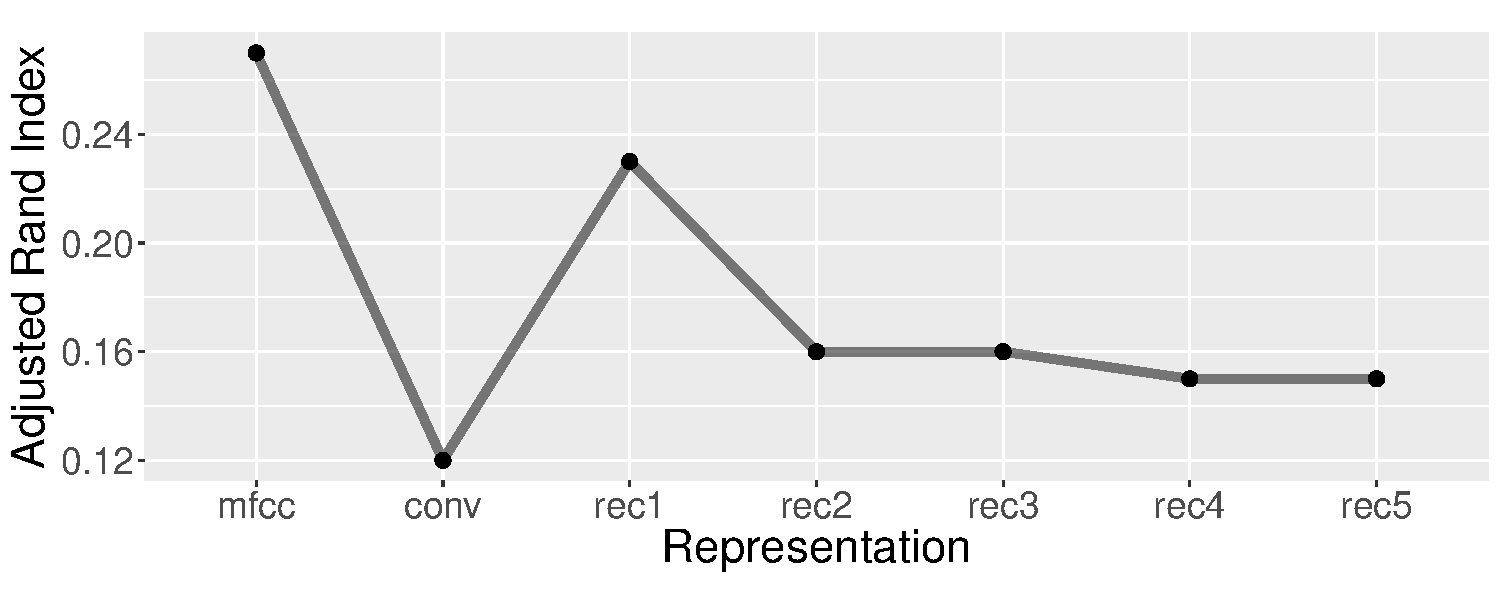
\includegraphics[scale=0.3]{figures/hier_ari.pdf}
  \caption{Adjusted Rand Index for the comparison of the phoneme type hierarchy induced from representations against phoneme classes.}
  \label{fig:hier_ari}
\end{figure}

We measured the adjusted Rand Index for the match between the
hierarchy induced from each representation against phoneme classes,
which were obtained by cutting the tree to divide the cluster into the
same number of classes as there are phoneme classes. There is a notable drop between the match from MFCC to the activation of the convolutional layer. We suspect this may be explained by the loss of information caused by averaging over phoneme instances combined with the lower temporal resolution of the activations compared to MFCC. The match improves markedly at recurrent layer~1.


\begin{figure*}[t]
  \centering
  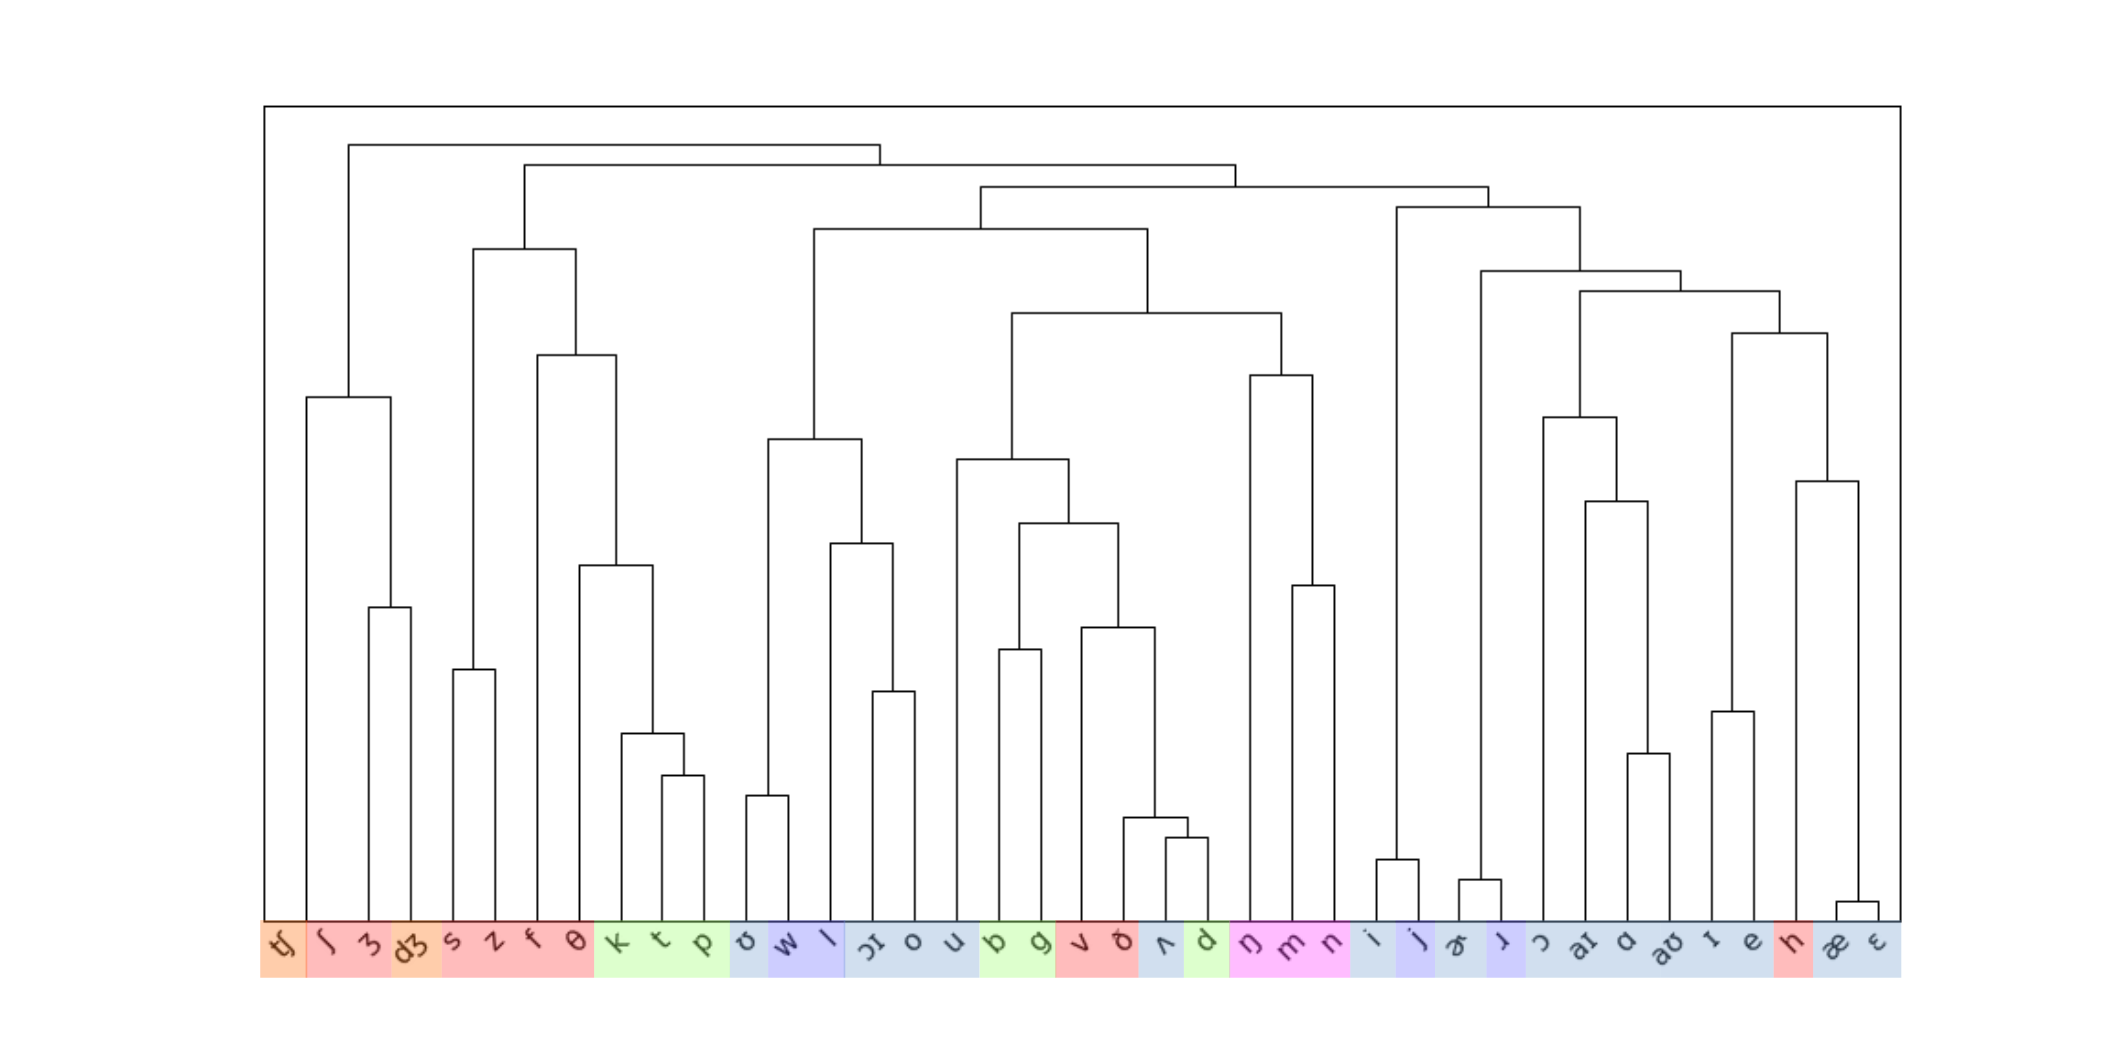
\includegraphics[scale=0.45]{figures/color-coded-activation0.png}
\caption{Hierarchical clustering of phoneme activation vectors on the first 
hidden layer.}
\label{fig:cluster-l0}
\end{figure*}



